\section{Feature Model}\label{ch:Feature Model}

%Reason for Feature model
A configurable system often contains numerous features, all of which may interact with one each other or have different dependencies.
However, as mentioned in \autoref{feature-config} not all features are freely combinable, some of them can only be selected in the
absence of others. The large the system the harder it gets to keep all these interactions in mind, therefore we use \emph{Feature Models}
to describe the relation between features and define which feature selections are valid \cite{Feature-Oriented-Software-Product-Lines}.

%Reason why featuremodel
Due to the fact that large configurable systems tends to have numerous feature we use feature diagrams which are a common
visual representation of feature models.

\subsection{Feature Diagram}

\begin{figure}[h]
    \centering
    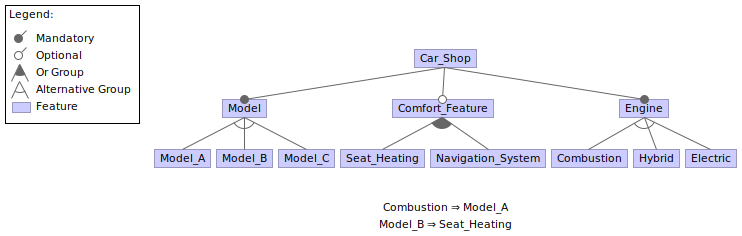
\includegraphics[scale=0.6]{gfx/Car_Shop.png}
    \caption{A feature diagram of a car dealership.}
    \label{fig:car}
\end{figure}

%What is a feature diagram and relation between features
A feature diagram is conceptually built as a tree where each node of the three represents a feature, 
where an edge between a parent node and a child usually implies that the parent is a more general concept and the child a specialization. 
This leads to the fact that the further we descent in the hierarchy of the diagram, the more specialized the feature gets.

%Feature diagram example
\autoref{fig:car} is an example for a feature diagram that depicts the structure of a car dealership. As we can see the root
is the first node \textit{car\_shop} represents the general concept. Now if we look at the child nodes of the
\textit{Engine} feature, we can see concrete engine types, such as \textit{Combustion}, \textit{Hybrid}, and \textit{Electric}.

%Concrete and abstract feature with example
We differentiate between two types of features, \emph{abstract} and \emph{concrete} features. 
Abstract features are used for structural purposes and do not correspond to implementation. 
In contrast, concrete features reflect variability inside the system.
In \autoref{fig:car}, the feature \textit{Engine} would be considered an abstract feature since it does not implement anything, and its purpose
is to group all types of engines the system contains. The specific engines, like \textit{Combustion} would be concrete features since
they implement a specific type of functionality.

%Mandatory and optional feature
Each feature contains a graphical notation indicating whether the feature is mandatory or optional. 
If the feature is mandatory, it is indicated with a black bubble; if it is optional, it is displayed with an empty bubble \cite{Feature-Oriented-Software-Product-Lines-Feature-models}. 
In \autoref{fig:car} we can see that \textit{Engine} and \textit{Model} are mandatory features, which make sense since both are necessary for any car, 
but \textit{Comfort\_Feature} an optional since they are not necessary for a car to function.

%Alternative and choice groups
In addition to mandatory and optional features, there are alternative and choice groups. 
A parent can have one of these groups; we mark an alternative group with an empty half circle and an optional group with a filled circle. 
When we use a selection group, one feature needs to be selected, but others can also be selected; a choice group corresponds to the logical or operator. 
In an alternative group, we can select only one feature; the configuration is invalid if more than one feature is selected \cite{Feature-Oriented-Software-Product-Lines-Feature-models}. 
In \autoref{fig:car}, we see that \textit{Engine} has an alternative group, which makes sense since each car can only contain one \textit{Engine}, 
whereas it makes sense that \textit{Comfort\_Feature} contains a choice group, you can have a navigation system and seat heating in a car without conflict.

%Constraints
A feature diagram may contain various constraints that need to be satisfied, defined as boolean algebra. In \autoref{fig:car}, we see two constraints, 
$Combustion \implies Model\_A$ and $Model\_B \implies Seat\_Heating$. The reason for such constraints could be that \textit{Model\_B} 
is a luxury model that only gets shipped with seat heating.

%Propositional formula , why useful
Any feature model can also be translated into propositional formula. Therefore, a
feature configuration is valid only iff it satisfies the propositional formula. We can therefore use a feature model to check whether a configuration 
is valid, which is particularly useful if we want to sample or enumerate all valid configurations \cite{Feature-Oriented-Software-Product-Lines-Feature-models}. 